\chapter{Экспериментальное обоснование метода неконтролируемого предобучения}

В данной главе приводится практическое обоснование теоретических результатов, описанных в главе 2, а именно, результаты сравнительного анализа методов предобучения и алгоритма редуцирования весовых коэффициентов нейросетевых моделей.

Для оценки эффективности предлагаемых методов применяются известные выборки данных, используемые для апробации подходов в области машинного обучения:
\begin{easylistNum}
    & выборка MNIST, представляющая собой набор из 70.000 черно-белых изображений рукописных цифр размерностью 28Х28 пикселей, представленных в виде одномерных векторов данных \cite{mnist};
    & выборка CIFAR-10, представляющая собой набор из 60.000 цветных изображений объектов 10 различных классов размерностью 32Х32 пикселя \cite{krizhevsky2009learning};
    & выборка CIFAR-100, представляющая собой набор из 60.000 цветных изображений объектов 100 различных классов размерность 32Х32 пикселя \cite{krizhevsky2009learning}.
\end{easylistNum}

Приводятся результаты экспериментальных исследований, полученных для задач сжатия данных, распознавания образов и редуцирования параметров ГНС.

Исходный код реализованных методов предобучения и редуцирования ИНС приводится в приложении \ref{app:a}.

%\section{Используемое программное и аппаратное обеспечение}

%Выполнение экспериментов с использованием выборок большого размера занимает достаточно продолжительное время. Эта проблема была решена проведением расчетов с использованием видеокарт nVidia, поддерживающих технологию CUDA (нами использовались ускорители A100 или V100, доступные при использовании сервиса Google Colab \cite{googlecolab}). Существуют другие способы ускорения расчетов, производимых при обучении нейронной сети, например, использование вычислительных кластеров \cite{n16}.

\section{Сжатие данных}

Для первоначальной оценки эффективности предлагаемого подхода предобучения глубокой нейронной сети, были проведены вычислительные эксперименты на искусственном наборе данных $\boldmath{x}$, лежащем на одномерном многообразии (спиральная петля), погруженном в трехмерное пространство \cite{n11} и генерируемом равномерно распределенным параметром $t \in [-1, 1]$:

\begin{equation*}
	\begin{cases}
		x_1=\sin(\pi t) + \mu\\
		x_2=\cos(\pi t) + \mu,\\
		x_3=t + \mu
	\end{cases}
\end{equation*}
где $\mu$ -- Гауссов шум со средним 0 и стандартным отклонением 0.05.

Для проверки предложенного метода, был обучен семислойный автоэнкодер, используя выборку из 1000 примеров. Глубокий автоэнкодер показан на рисунке \ref{fig:autoencoder}. Мы использовали логистические функции активации для всех слоев нейронной сети, за исключением среднего слоя (<<узкого места>>). На этом слое использовалась линейная функция активации.

\begin{figure}[ht]
	\centering
	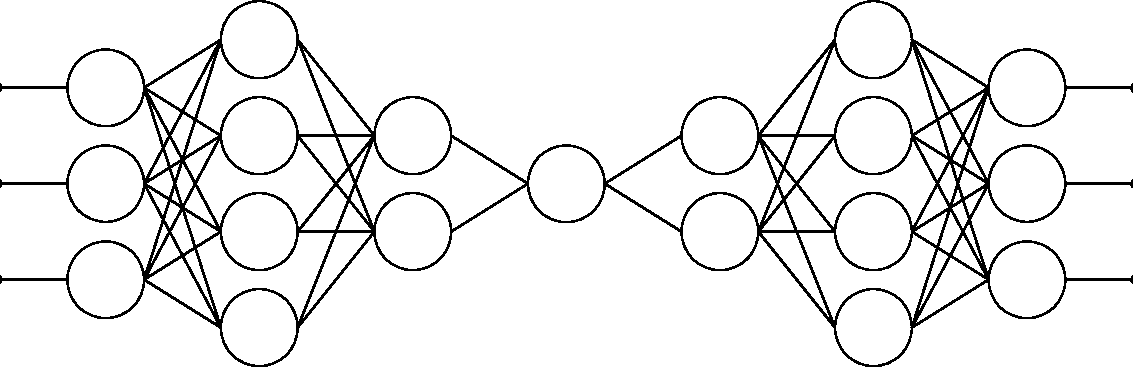
\includegraphics[width=16cm]{man-source/images/ch3/pic3-5.pdf}
	\caption{Глубокий автоэнкодер}
	\label{fig:autoencoder}
\end{figure}

Результаты обучения показаны в таблице \ref{table:data_compressing}. Здесь MSE -- среднеквадратичная ошибка на выборке обучения, MS -- среднеквадратичная ошибка на тестовой выборке для проверки обобщающей способности сети. Количество примеров в тестовой выборке -- 1000. Скорость обучения $\alpha$ -- 0.1 для классического метода обучения и 0.5 для REBA для всех экспериментов.

			\begin{table}[h]
				\caption{Сравнение методов предобучения (сжатие)}								\label{table:data_compressing}
				\centering
				\begin{tabular}{|p{4cm}|p{3cm}|p{2cm}|p{2cm}|}
					\hline
					Метод & CD-k & MSE & MS \\
					\hline
					C-RBM & 1  & 0,699 & 0,886 \\
                        \cline{2-4}
					& 5  & \textbf{0,710} & \textbf{0,932}\\
                        \cline{2-4}							
					&	10 & 0,689 & 0,916\\
					\cline{2-4}
                        &	15 & \textbf{0,688} & \textbf{0,873}\\ \hline
					REBA& 1  & \textbf{0,673} & \textbf{0,851}\\
                        \cline{2-4}
					& 5  & 0,719 & 0,966\\
                        \cline{2-4}
					&	10 & \textbf{0,677} & \textbf{0,907}\\
                        \cline{2-4}
					&	15 & 0,700 & 0,895 \\						
					\hline
				\end{tabular}			
			\end{table}	

Число эпох предобучения -- 10. Число эпох <<тонкой настройки>> нейронной сети -- 1000. Из полученных результатов видно, что использование метода предобучения REBA позволило улучшить обобщающую способность глубокого автоэнкодера для случаев CD-1 и CD-10. На рисунках \ref{f:15} и \ref{f:16} изображены оригинальные данные, на которых производилось обучение, и восстановленные из одного нелинейного компонента, используя тестовые данные. Как можно видеть, автоэнкодер восстанавливает данные из одного нелинейного компонента с хорошей точностью.

\begin{figure}[h]
	\begin{center}
		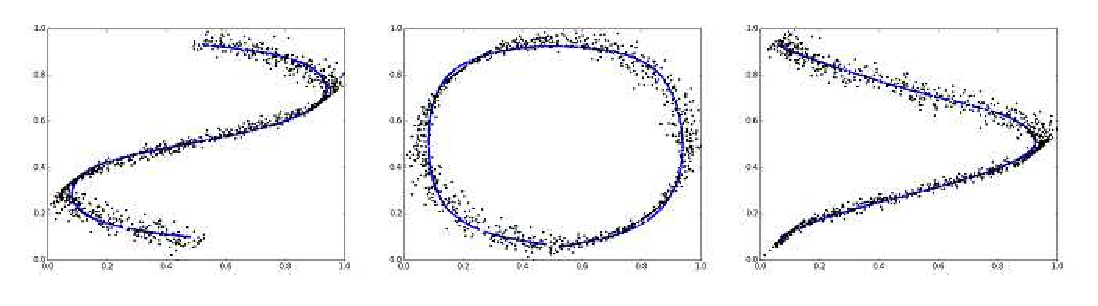
\includegraphics[width=160mm]{man-source/images/ch3/pic3-6.pdf}
		\caption{2D-изображения оригинальных и реконструированных данных}				
		\label{f:15}
	\end{center}
\end{figure}

\begin{figure}[h!]
	\begin{center}
		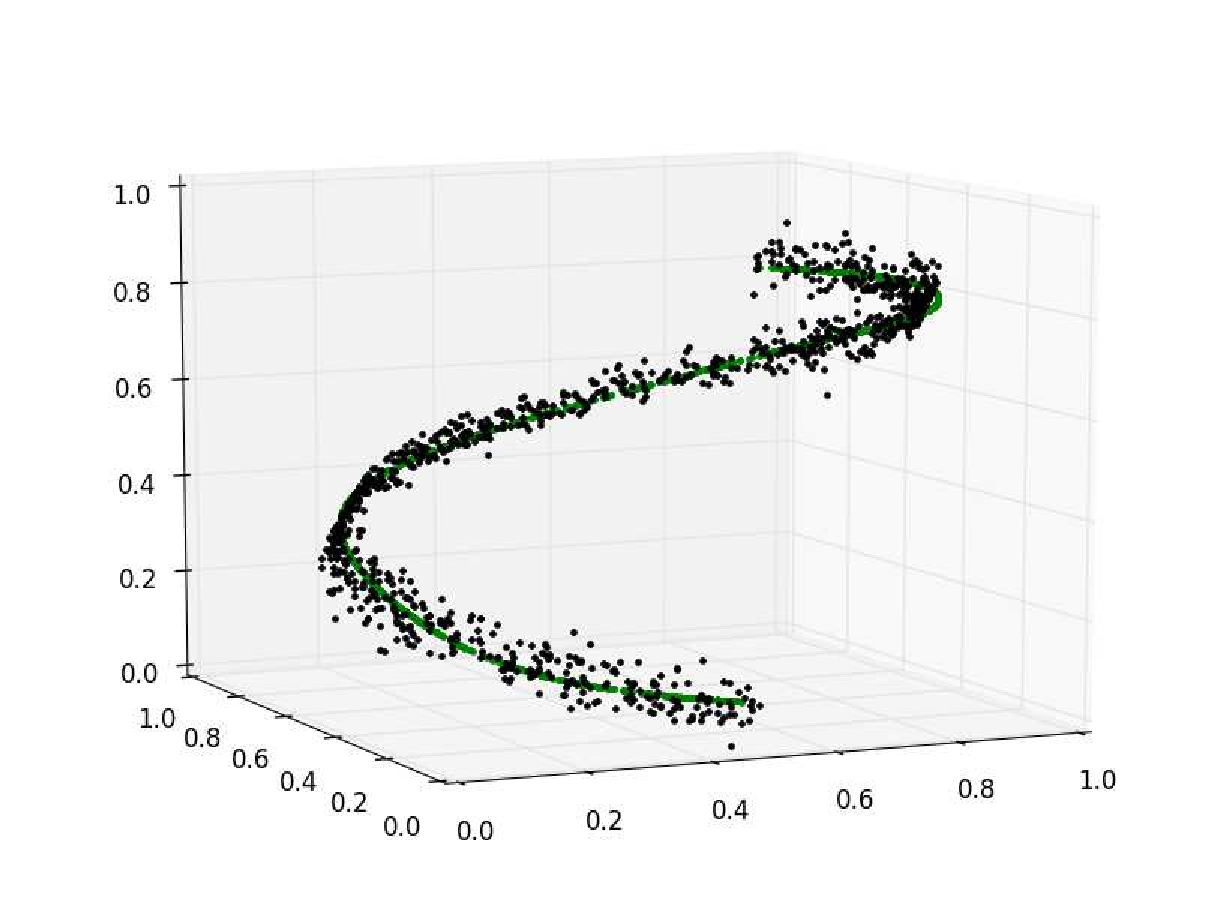
\includegraphics[width=120mm]{man-source/images/ch3/pic3-7.pdf}
		\caption{3D-изображение оригинальных и реконструированных данных}				
		\label{f:16}
	\end{center}
\end{figure}

% \section{Распознавание образов}
% \subsection{Ирисы Фишера}

% Рассмотрим решение задачи распознавания образов на примере известной выборки Фишера \cite{Fisher}. Эта выборка была представлена Рональдом Фишером в 1936 году в качестве примера для демонстрации разработанного им метода линейного дискриминантного анализа. Она включает 150 образов ирисов, относящихся к трем различным классам. Каждый образ представляет собой 4-х мерный вектор признаков.

% Отличительная особенность этой задачи в том, что один класс образов является линейно разделимым, в то время как два других -- нет (рис. \ref{fig:irises_visualize}).

% \begin{figure}[h]
% 	\begin{center}
% 		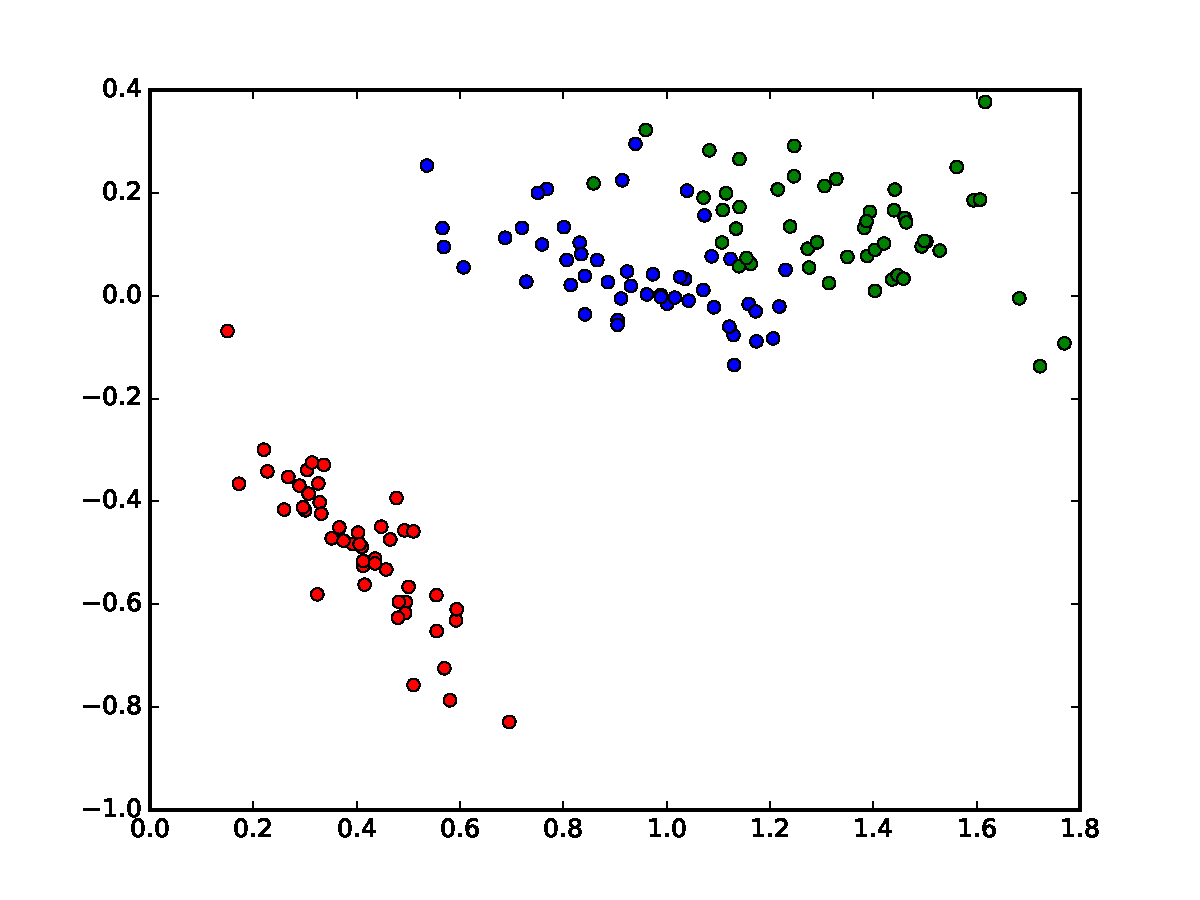
\includegraphics[width=10cm]{man-source/images/ch3/pic3-8.pdf}
% 		\caption{Визуализация образов ирисов Фишера (получена применением PCA)}				
% 		\label{fig:irises_visualize}
% 	\end{center}
% \end{figure}

% Применяя классические подходы кластеризации (например, метод k-средних), можно заметить неприемлемое качество распознавания на границах двух линейно неразделимых классов (рис. \ref{fig:kmeans})

% \begin{figure}[h]
% 	\begin{center}
% 		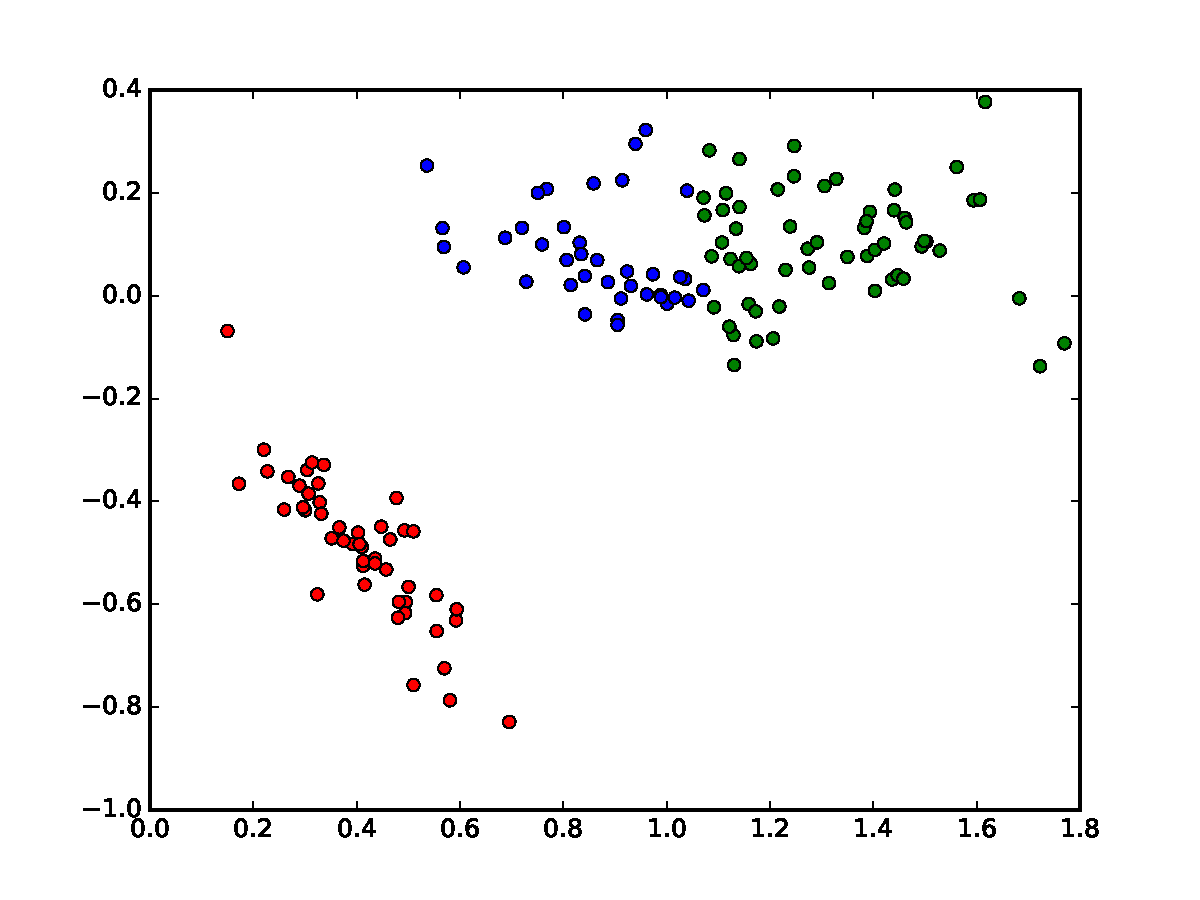
\includegraphics[width=10cm]{man-source/images/ch3/pic3-9.pdf}
% 		\caption{Кластеризация образов ирисов Фишера методом k-средних}			
% 		\label{fig:kmeans}
% 	\end{center}
% \end{figure}

% Обучим глубокую нейронную сеть для классификации образов из выборки Фишера. Для решения этой задачи воспользуемся сетью с архитектурой \textbf{4-32-16-8-3} с сигмоидными функциями активации на каждом обрабатывающем слое. 
% Другие параметры:
% \begin{itemize}
% 	\item Фаза предобучения: скорость -- 0.1 (для REBA 0.4), моментный параметр -- переменный (от 0.5 до 0.9), размер мини-батча - 5, количество эпох обучения каждого слоя -- 50.
% 	\item Фаза обучения: скорость -- 0.05 (с редуцированием, коэффициент 0.99), моментный параметр -- 0.9, размер мини-батча -- 5, количество эпох обучения -- 2000, параметр L2-регуляризации (weight decay) -- 0.00001.
% \end{itemize}

% После обучения нейронной сети нами была достигнута совокупная ошибка распознавания 99,33\%. Таким образом, неправильно распознанным остался только один образ из всей выборки (см. рис. \ref{fig:fisher_irises_results}).

% \begin{figure}[h]
% 	\begin{center}
% 		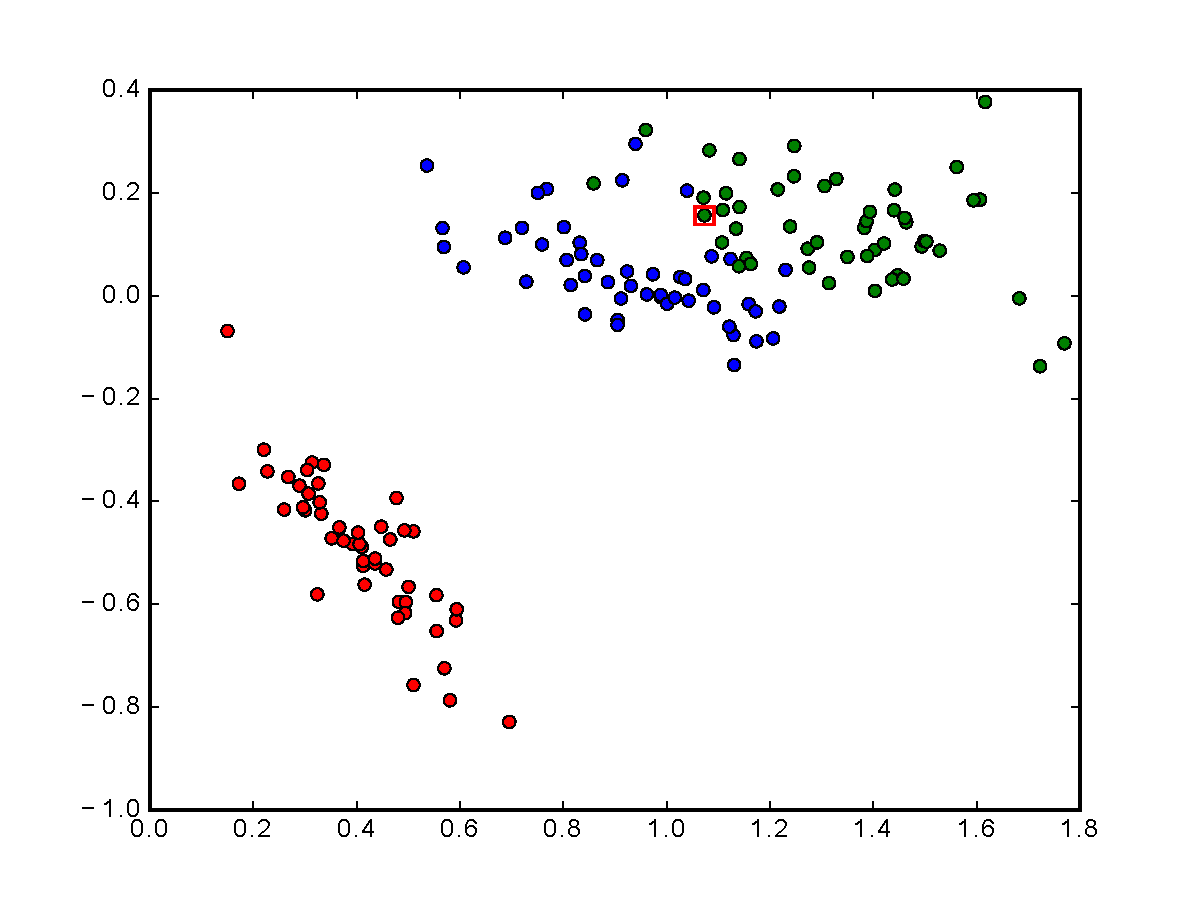
\includegraphics[width=12cm]{man-source/images/ch3/pic3-10.pdf}
% 		\caption{Результат работы обученной глубокой нейронной сети с отмеченным неправильно классифицированным образом}				
% 		\label{fig:fisher_irises_results}
% 	\end{center}
% \end{figure}

% Показательной в данном случае является эволюция среднеквадратичной ошибки после предобучения разными методами и без него (рис. \ref{fig:error_evolution}).

% \begin{figure}[h]
% 	\begin{center}
% 		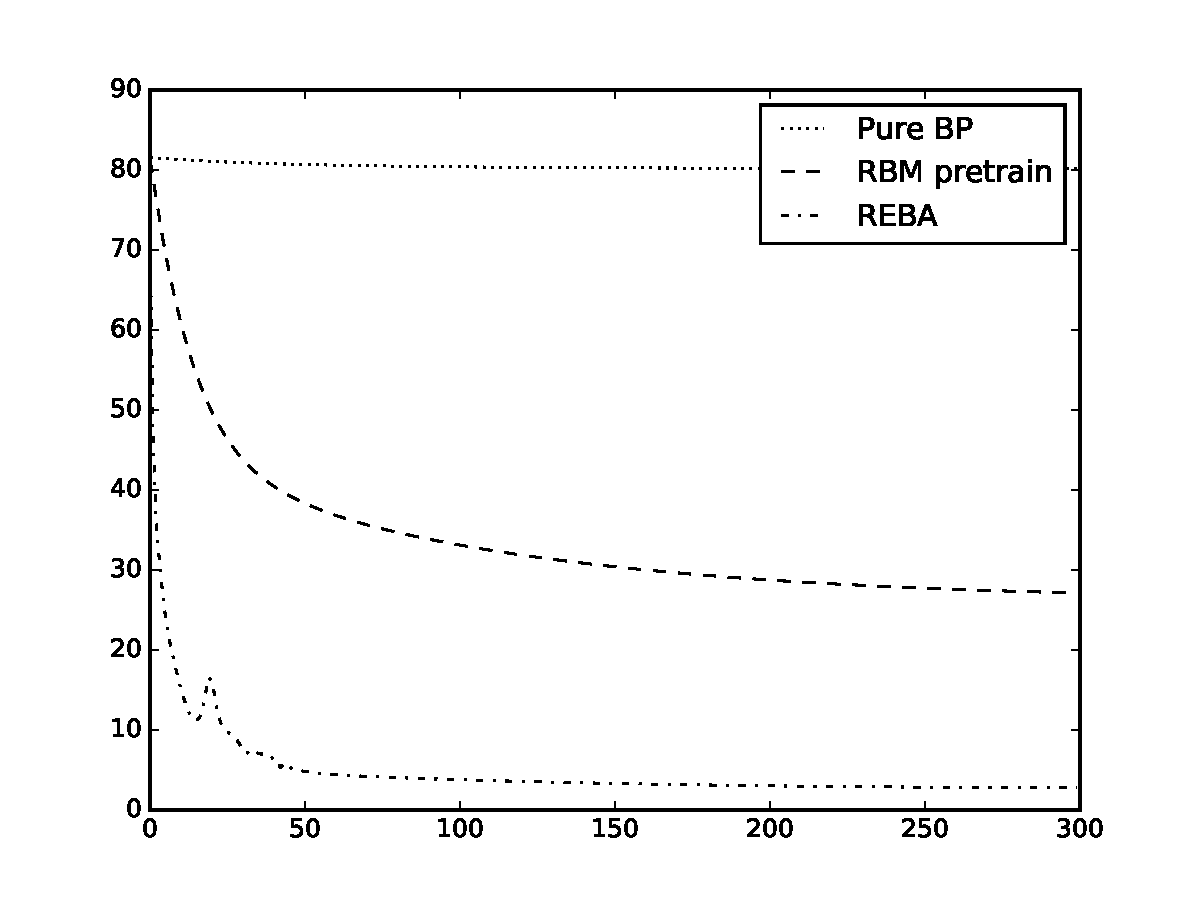
\includegraphics[width=12cm]{man-source/images/ch3/pic3-11.pdf}
% 		\caption{Эволюция ошибок обучения разными методами}	
% 		\label{fig:error_evolution}
% 	\end{center}
% \end{figure}

% Таким образом, предобучение позволяет получить хорошую начальную инициализацию весов и порогов нейронной сети, что делает последующий этап <<тонкой настройки>> методом обратного распространения ошибки значительно более продуктивным.

% \section{Гибридный алгоритм предобучения}

% При обучении нейронных сетей, как поверхностных, так и глубоких архитектур, можно использовать целевые минимизируемые функции разных видов. В главе 1 были приведены основные функции ошибок, часто применяемые на практике (\ref{MSE}, \ref{CE}).

% В различных публикациях исследуется вопрос применения обоих критериев (например, \cite{Golik}, \cite{Zhou}). При этом полученные в \cite{Golik} результаты подтверждают, что обучение классификаторов в соответствии с критерием $E_{CE}$ позволяет найти лучший локальный оптимум, чем с критерием $E_{MSE}$, применение которого приводит к быстрому <<застреванию>> в локальном оптимуме, где градиент стремится к нулю и, как результат, дальнейшее уменьшение ошибки классификации становится невозможным. 

% В \cite{Golik} исследуется вопрос применения гибридного подхода. Начиная с хорошей начальной инициализации, полученной при обучении с критерием $E_{CE}$, дальнейший процесс с $E_{MSE}$ способен дать лучший результат, чем при обучении только с критерием $E_{CE}$. 

% % При этом полученные авторами результаты подтверждают, что если обучение вначале будет вестись в соответствии с правилами по формуле $E_{CE}$, а затем несколько эпох - по формуле $E_{MSE}$, итоговая обобщающая способность сети будет выше, чем при обучении только с использованием $E_{CE}$.

% Таким образом, с учетом ранее доказанных теорем, может быть сформулирован гибридный вариант предобучающего алгоритма.

\section{Распознавание образов}

\subsection{Критерий оценки результатов классификации}

Для оценки качества решения задачи классификации применялся следующий подход. Вначале определялся $k$-тый нейрон, выходное значение которого было максимальным для заданного образа $s$ (данное число соответствует метке класса, получаемого моделью):

\begin{equation}
  k_s = \arg \max_j y_j^s.
\end{equation}

Затем получившееся значение сравнивалось с эталонными значениями и количество совпадений суммировалось для всех образов:

\begin{equation}
  S = \sum_{s=1}^{L} [k_s = e_s],
\end{equation}
где $[x]$ -- нотация (скобка) Айверсона для высказывания $x$,\\
$L$ -- общее количество образов из оцениваемого множества,\\
$e_s$ -- эталонное значение, метка класса, соответствующая $s$-тому образу.

Значения нотации Айверсона могут быть получены по следующей формуле:

\begin{equation*}
    [x] = 
    \begin{cases}
        1, & \text{x is True} \\
        0, & \text{x is False}.
    \end{cases}
\end{equation*}

Таким образом, общая эффективность на тестовой выборке может быть получена по следующей формуле:

\begin{equation}
\text{Efficiency} = \frac{S}{L} * 100\%.
\end{equation}

\subsection{Ирисы Фишера}

Рассмотрим решение задачи распознавания образов на примере известной выборки Фишера \cite{Fisher}. Эта выборка была представлена Рональдом Фишером в 1936 году в качестве примера для демонстрации разработанного им метода линейного дискриминантного анализа. Она включает 150 образов ирисов, относящихся к трем различным классам. Каждый образ представляет собой 4-х мерный вектор признаков.

Отличительная особенность этой задачи в том, что один класс образов является линейно разделимым, в то время как два других -- нет (рисунок~\ref{fig:irises_visualize}).

\begin{figure}[h]
	\begin{center}
		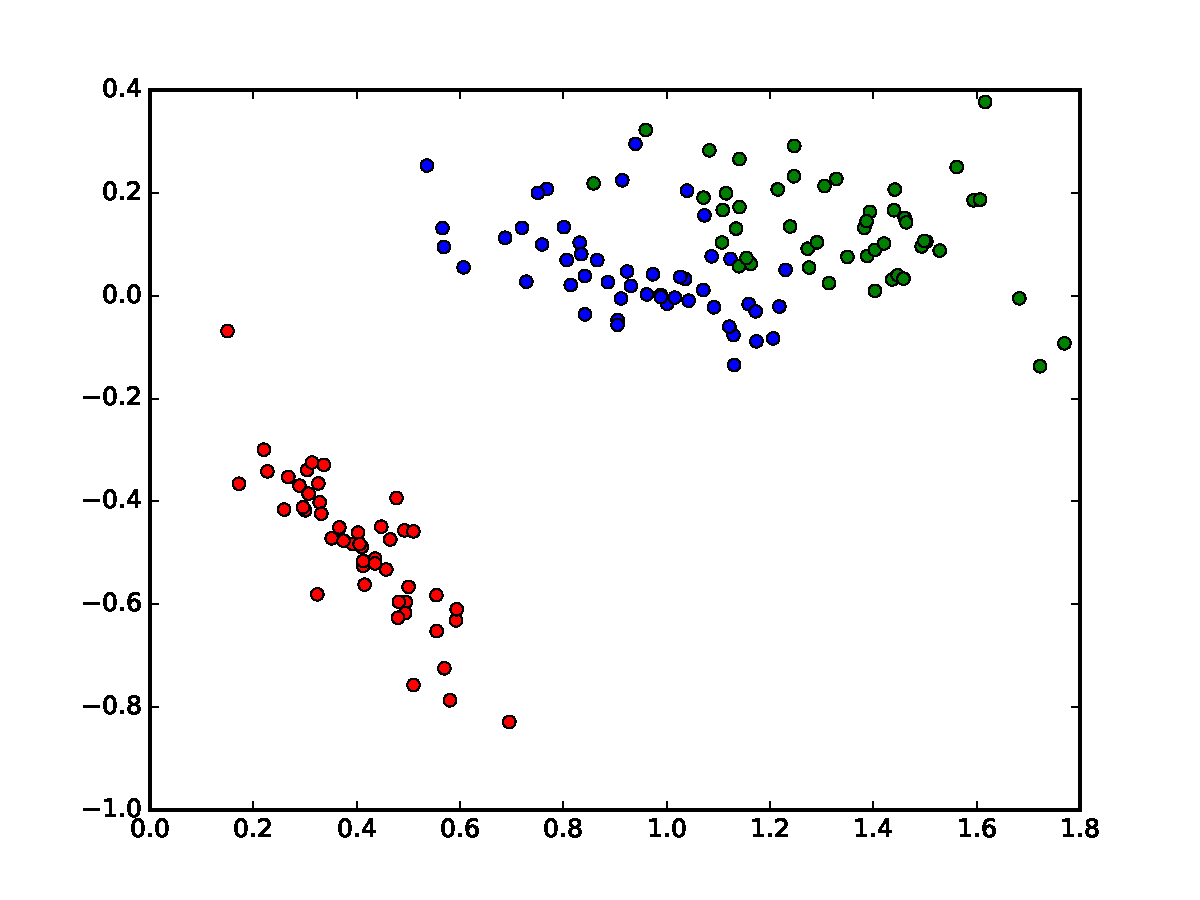
\includegraphics[width=10cm]{man-source/images/ch3/pic3-8.pdf}
		\caption{Визуализация образов ирисов Фишера (получена применением метода PCA)}				
		\label{fig:irises_visualize}
	\end{center}
\end{figure}

Применяя классические подходы кластеризации (например, метод k-средних), можно заметить неприемлемое качество распознавания на границах двух линейно неразделимых классов (рисунок \ref{fig:kmeans}).

\begin{figure}[h]
	\begin{center}
		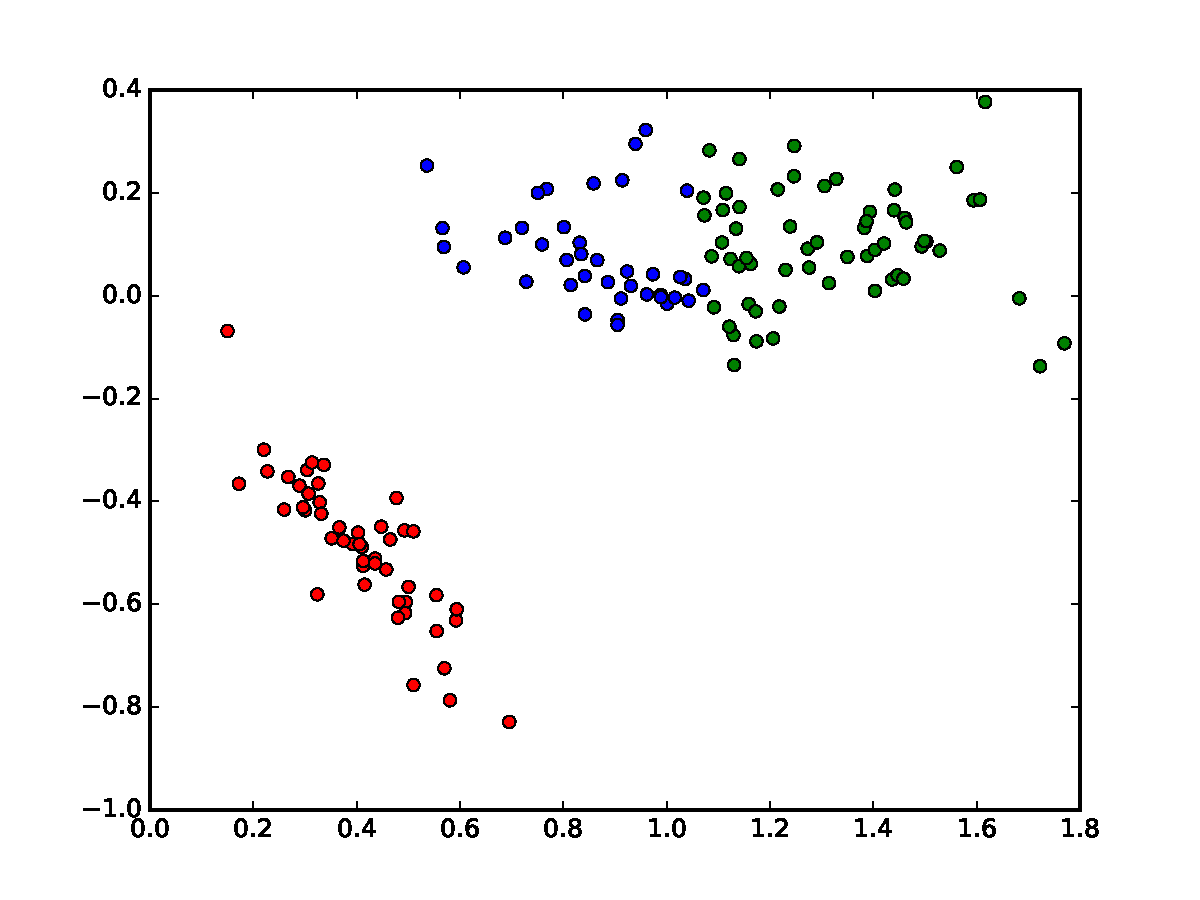
\includegraphics[width=10cm]{man-source/images/ch3/pic3-9.pdf}
		\caption{Кластеризация образов ирисов Фишера методом k-средних}			
		\label{fig:kmeans}
	\end{center}
\end{figure}

Для решения этой задачи была использована сеть с архитектурой \textbf{4-32-16-8-3} с сигмоидными функциями активации на каждом обрабатывающем слое. 
Другие параметры:
\begin{itemize}
	\item фаза предобучения: скорость -- 0.1 (для REBA 0.4), моментный параметр -- переменный (от 0.5 до 0.9), размер мини-батча - 5, количество эпох обучения каждого слоя -- 50;
	\item фаза обучения: скорость -- 0.05 (с редуцированием, коэффициент 0.99), моментный параметр -- 0.9, размер мини-батча -- 5, количество эпох обучения -- 2000, параметр L2-регуляризации (weight decay) -- 0.00001.
\end{itemize}

После обучения нейронной сетью была достигнута совокупная ошибка распознавания 99,33\%. Таким образом, неправильно распознанным остался только один образ из всей выборки (рисунок \ref{fig:fisher_irises_results}).

\begin{figure}[h]
	\begin{center}
		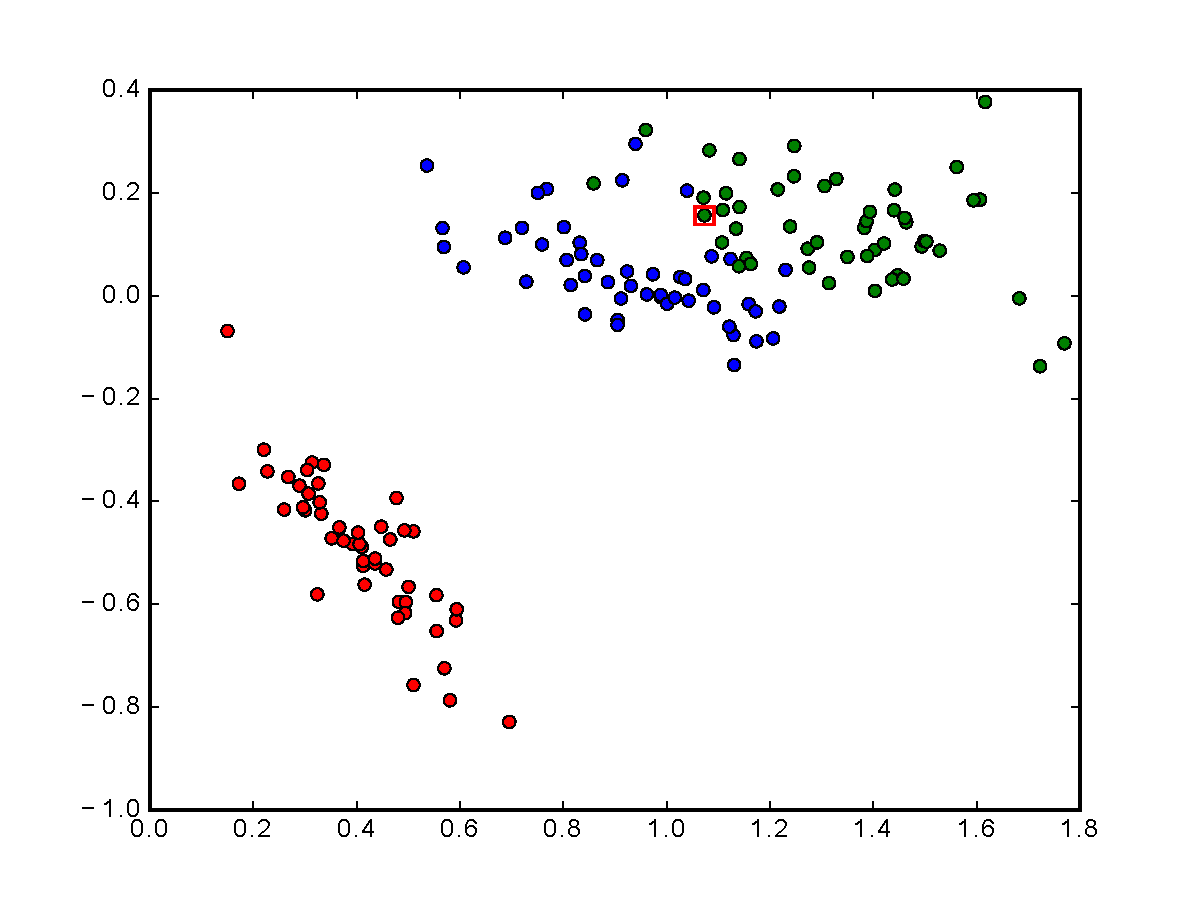
\includegraphics[width=12cm]{man-source/images/ch3/pic3-10.pdf}
		\caption{Результат работы обученной нейронной сети с отмеченным неправильно классифицированным образом}				
		\label{fig:fisher_irises_results}
	\end{center}
\end{figure}

Эволюция среднеквадратичной ошибки после предобучения разными методами и без предобучения изображена на рисунке \ref{fig:error_evolution}.

\begin{figure}[h]
	\begin{center}
		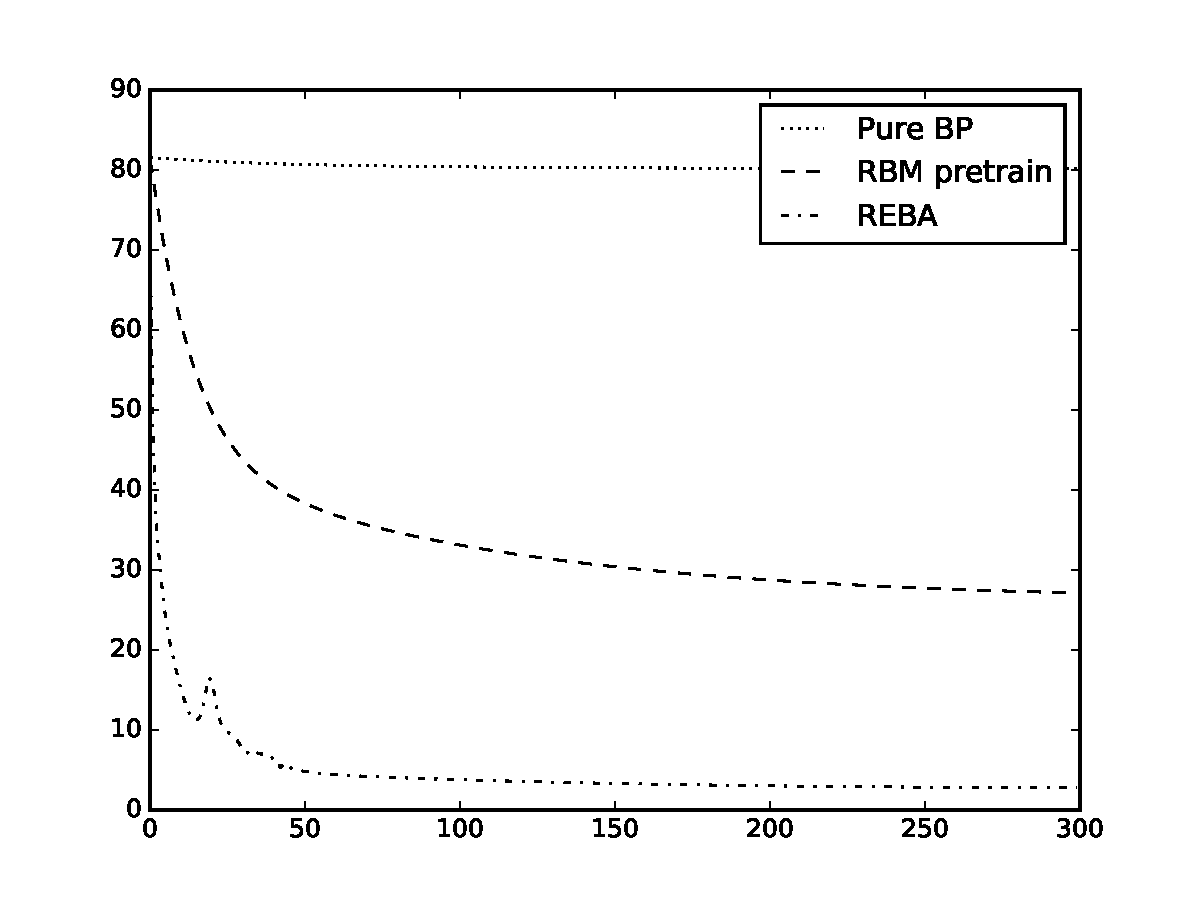
\includegraphics[width=12cm]{man-source/images/ch3/pic3-11.pdf}
		\caption{Эволюция ошибок обучения разными методами}	
		\label{fig:error_evolution}
	\end{center}
\end{figure}

Как видно из представленного графика, предобучение позволяет получить хорошую начальную инициализацию весов и порогов нейронной сети, что делает последующий этап <<тонкой настройки>> методом обратного распространения ошибки более эффективным.

\subsection{Описание выборок}

С практической точки зрения (и в соответствии с объектом исследования) наибольший интерес представляют выборки графических образов.

Задача распознавания графических образов является одной из основных в области компьютерного зрения. В настоящий момент <<золотым стандартом>> выборок, применяемых для оценки эффективности моделей выступают MNIST, CIFAR-10 и CIFAR-100. %На этих выборках уже получены хорошие результаты по достигнутой эффективности моделей. Однако, нужно отметить, что для ряда подходов, для которых получены лучшие результаты при тестировании на данных выборках, используются аугментированные (т.е. измененные данные), которые позволяют значительно увеличить размерность обучающей выборки. Перед нами стояла задача сравнения методов предобучения, без достижения state-of-art результатов для выборок, поэтому методы аугментации данных не применялись.

Выборка MNIST (Mixed National Institute of Standards and Technology database) является классической при тестировании систем распознавания образов, а также широко используемой для обучения и тестирования алгоритмов машинного обучения. Она сформирована как подмножество более крупной оригинальной выборки NIST \cite{mnist}, изображения из которого были дополнительно предобработаны (путем изменения размера и центрирования). 

Выборка MNIST состоит из 60000 образов для обучения и 10000 образов для тестирования. Каждый образ представляет собой изображение цифры размером 28Х28 пикселей в градациях серого цвета. На рисунке \ref{fig:mnist_example} изображен фрагмент базы изображений MNIST с наиболее труднораспознаваемыми цифрами.

\begin{figure}[h]
	\begin{center}
		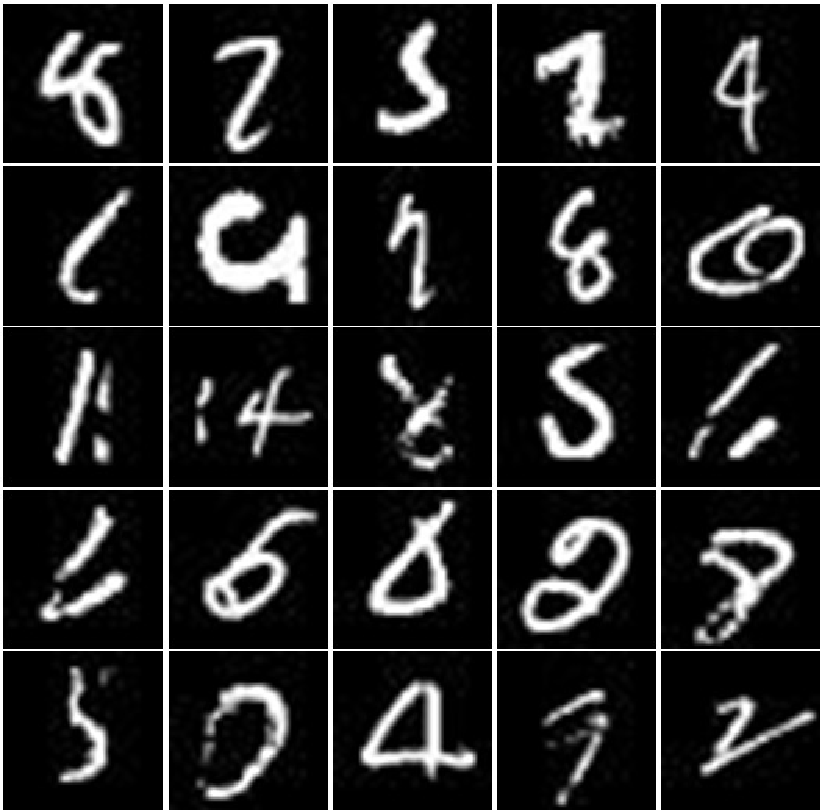
\includegraphics[width=8cm]{man-source/images/ch3/pic3-12.pdf}
		\caption{Фрагмент базы изображений MNIST}		
		\label{fig:mnist_example}
	\end{center}
\end{figure}

Выборка CIFAR-10 \cite{krizhevsky2009learning} является подмножеством выборки Tiny Images \cite{torralba2008} и включает в себя 60.000 цветных изображений технических средств и живых существ, принадлежащий 10 различным классам (рисунок~\ref{fig:cifar_dataset}) по 6.000 изображений на каждый класс. Каждое изображение имеет размер 32Х32 пикселя.

\begin{figure}[h!]
	\begin{center}
		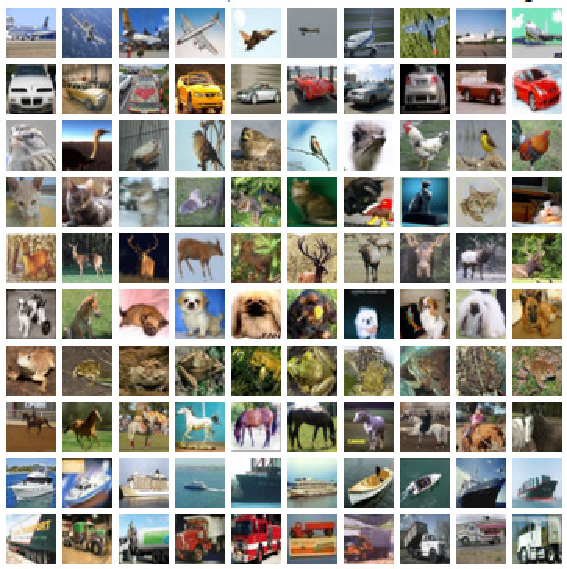
\includegraphics[width=10cm]{man-source/images/ch3/pic3-2.pdf}
		\caption{Фрагмент базы изображений CIFAR-10}				
		\label{fig:cifar_dataset}
	\end{center}
\end{figure}

Выборка CIFAR-100 идентична выборке CIFAR-10 по параметрам изображений, которые в нее включены, но отличается количеством представленных классов изображений (в этой выборке общее количество классов составляет 100). Общая размерность выборки составляет также 60.000~изображений, по 600 изображений на каждый класс.

Выборки CIFAR-10 и CIFAR-100 разделены авторами на обучающую и тестовую подвыборки (объемом 50.000 и 10.000 изображений соответственно).

%Выполнение экспериментов с использованием выборок большого размера занимает достаточно продолжительное время. Эта проблема может быть решена проведением расчетов с использованием видеокарт nVidia, поддерживающих технологию CUDA (например, ускорителей A100 или V100, доступных при использовании сервиса Google Colab \cite{googlecolab}). Существуют другие способы ускорения расчетов, производимых при обучении нейронной сети, например, использование вычислительных кластеров \cite{n16}.

%Количество входов обучаемой НС определялось размерами образов из базы MNIST (784), количество слоев и нейронов в каждом слое выявлялось экспериментальным путем. На каждом слое использовалась сигмоидная функция активации. 

\subsection{Параметры вычислительного эксперимента и результаты}

В качестве целевой модели для решения задачи распознавания изображений из выборки MNIST была выбрана сверточная нейронная сеть с параметрами, представленными в таблице \ref{table:mnist_conv_model}.

\begin{table} [!h]
  \caption{MNIST: основные параметры используемой модели}\label{table:mnist_conv_model}
\centering
\begin{tabular}{| p{7cm} | p{8cm} |}
  \hline
    \textbf{Параметр} & \textbf{Значение}\\
    \hline
    Архитектура & 40Х5Х5 -- 40Х5Х5 -- 640Х320 -- 320Х160 -- 160Х10\\
    \hline
    Функция активации & ReLU \\
    \hline
    Функция активации на последнем слое & Softmax \\
    Начальная инициализация параметров & Нормальное распредение \\
    \hline
\end{tabular}
\end{table}

Первые (сверточные) слои обозначены условно как \textit{K} x \textit{S} x \textit{S}, где \textit{K} обозначает количество ядер свертки в соответствующем слое, a \textit{S} x \textit{S} -- размерность ядра свертки.

Как видно из представленной выше таблицы, использовалась архитектура с 5 обрабатывающими слоями, 2 из которых сверточные, а 3 -- полносвязные. При этом общее число параметров модели составило 299.170.

В качестве функции активации использовалась функция ReLU на всех слоях сети, за исключением последнего слоя, на котором применялась softmax-функция. Использование ReLU позволило варианту обучения без предобучения начать процесс и завершить его с приемлемым значением эффективности.

В таблице \ref{table:mnist_comparing_params} приведены основные используемые параметры обучения.

Помимо классического и предложенного методов предобучения в ходе проведения экспериментов был протестирован подход, при котором первый слой нейросетевой модели предобучается с использованием классического метода обучения RBM, а все прочие слои, кроме последнего классифицирующего -- с использованием предлагаемого подхода REBA. Будем обозначать такой вариант предобучения как гибридный (HREBA).

Эксперименты проводились с одной и той же начальной инициализацией параметров для всех методов серией в 10 попыток, получаемые результаты затем усреднялись. В ходе эксперимента сравнивались четыре основных варианта обучения: 
\begin{easylistNum}
    & BP -- обучение без предобучения; 
    & REBA -- обучение с предобучением (предлагаемый подход); 
    & HREBA -- обучение с предобучением (гибридный подход);
    & C-RBM -- обучение с классическим методом предобучения).
\end{easylistNum}

\begin{table} [!h]
  \caption{MNIST: основные параметры обучения}\label{table:mnist_comparing_params}
\centering
\begin{tabular}{| p{3cm} | p{6cm} | p{2.5cm} |}
  \hline
    \textbf{Этап} & \textbf{Параметр} & \textbf{Значение}\\
    \hline
    Предобучение & Скорость обучения & 0,000125\\
    \cline{2-3}
    & Размер мини-батча & 128 \\
    \cline{2-3}
    & Моментный параметр & [0,5; 0,9] \\
    \cline{2-3}
    & Количество эпох обучения & 30\\
    \hline
    Обучение & Скорость обучения & 0,001\\
    \cline{2-3}
    & Размер мини-батча & 128 \\
    \cline{2-3}
    & Моментный параметр & 0,9 \\
    \cline{2-3}
    & Количество эпох обучения & 50\\
    \hline
\end{tabular}
\end{table}

В результате были получены показатели эффективности для вышеперечисленных методов, представленные в таблице \ref{table:mnist_results}.

\begin{table} [!h]
  \caption{MNIST: результаты обучения}\label{table:mnist_results}
\centering
\begin{tabular}{| p{6cm} | p{6cm} |}
  \hline
    \textbf{Метод обучения} & \textbf{Эффективность, \%}\\
    \hline
    BP & 99.367\\
    \hline
    REBA & 99.371\\
    \hline
    HREBA & \textbf{99.458}\\
    \hline
    C-RBM & 99.447\\
    \hline
\end{tabular}
\end{table}

Как видно из представленных результатов, лучший средний показатель был достигнут гибридным методом HREBA, сочетающим в себе предобучение классическим и предложенным подходом, при этом максимальная эффективность была получена этим же методом и составила \textbf{99.53} \%.

При проведении экспериментов с выборками CIFAR-10 и CIFAR-100 использовалась модель с архитектурой, представленной в таблице \ref{table:cifar_comparison_params}.

Для выборки CIFAR-100 изменения в архитектуре модели коснулись только последнего слоя (вместо 10 выходных нейронов использовалось 100 -- по количеству классов в данной выборке).

\begin{table}[!h]
    \caption{CIFAR-10/CIFAR-100: основные параметры используемых моделей}\label{table:cifar_comparison_params}
    \begin{tabular}{|p{7cm}|p{8cm}|}
        \hline
        \textbf{Параметр} & \textbf{Значение}\\
        \hline
        Архитектура & 64Х5Х5 -- 32Х5Х5 -- 800Х128 -- 128Х10/100\\
        \hline
        Функция активации & ReLU - Tanh - ReLU \\
        \hline
        Функция активации на последнем слое & Softmax \\
        \hline
        Начальная инициализация параметров & Нормальное распредение \\
        \hline
        Общее число параметров модели & 159.914
        \\
        \hline
    \end{tabular}
\end{table}

В результате были получены показатели эффективности для вышеперечисленных методов, представленные в таблице \ref{table:cifar_10_results} (для выборки CIFAR-10) и \ref{table:cifar_100_results} (для выборки CIFAR-100).

\begin{table} [!h]
  \centering
  \caption{CIFAR-10: результаты обучения}\label{table:cifar_10_results}
  \begin{tabular}{| p{6cm} | p{6cm} |}
    \hline
      \textbf{Метод обучения} & \textbf{Эффективность, \%}\\
      \hline
      BP & 69.74\\
      \hline
      REBA & 71.20\\
      \hline
      HREBA & \textbf{71.59}\\
      \hline
      C-RBM & 71.51\\
      \hline
  \end{tabular}
\end{table}

Лучший результат был получен методом HREBA и составил \textbf{72.32\%}.

\begin{table} [!h]
  \centering
  \caption{CIFAR-100: результаты обучения}\label{table:cifar_100_results}
  \begin{tabular}{| p{6cm} | p{6cm} |}
    \hline
      \textbf{Метод обучения} & \textbf{Эффективность, \%}\\
      \hline
      BP & 36.83\\
      \hline
      REBA & 38.9\\
      \hline
      HREBA & \textbf{39.86}\\
      \hline
      C-RBM & 39.71\\
      \hline
  \end{tabular}
\end{table}

Лучший результат также был получен методом HREBA и составил \textbf{40.26\%}.

% Мы использовали следующие параметры обучения: скорость обучения -- 0,1 для REBA и 0,2 для классического метода RBM, размер мини-батча -- 100, количество эпох предобучения -- 10, количество эпох <<тонкой>> настройки -- 100. Также мы использовали параметр регуляризации L2, равный 0,00001.

% Результаты экспериментов представлены в таблице \ref{table:tbl2}. \textbf{MSE} определяет ошибку обучения, \textbf{MS} -- ошибку обобщения, \textbf{Ошибка, \%}, \% -- процент ошибочно распознанных изображений, \textbf{К-во эпох} -- число эпох для классического и гибридного метода предобучения.

% \begin{table}[H]
% 	\caption{Сравнение методов предобучения (MNIST)}
% 	\label{table:tbl2}
% 	\centering
% 	\begin{tabularx}{\hsize}{| c | c | c | c | X |}
% 		\hline
% 		\textbf{Метод} & \textbf{MSE} & \textbf{MS} & \textbf{Ошибка, \%} & \textbf{Кол-во эпох}\\
% 		\hline
% 		Classic RBM & 6,178e-6  & 0,0235 & 1,23 & 10 \\
% 		\hline
% 		Hybrid REBA (9+1) & 5,962e-6 & 0,0224 & \textbf{1,09} & 9+1 \\										
% 		\hline
% 	\end{tabularx}			
% \end{table}	

% Необходимо отметить, что нейронная сеть обученная на полной выборке из базы MNIST, ошибается на образах, многие из которых трудноразличимы даже для человеческого глаза (рис. \ref{fig:incorrect_recognized_samples})

% \begin{figure}[h]
% 	\begin{center}
% 		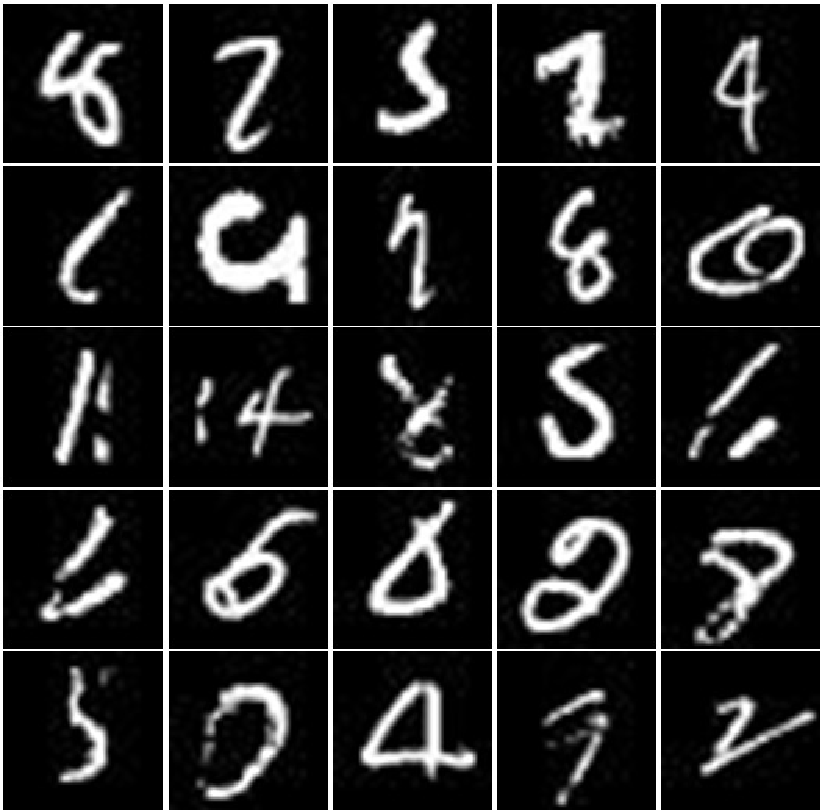
\includegraphics[width=8cm]{man-source/images/ch3/pic3-12.pdf}
% 		\caption{Образы, некорректно распознанные НС}		
% 		\label{fig:incorrect_recognized_samples}
% 	\end{center}
% \end{figure}

% \section{Визуализация данных}

% Для иллюстрации производительности метода REBA мы провели эксперименты по визуализации данных выборки MNIST. Для отображение 784-мерных данных, соответствующих количеству пикселей в исходном выражении нами использовался глубокая автоассоциативная сеть с архитектурой 784-500-500-250-10-2. Для всех слоев, за исключением среднего слоя, использовалась сигмоидная функция активации. На среднем слое применялась линейная функция. 

% Вначале выполнялось предобучение в соответствии с <<жадным>> послойным алгоритмом. Затем выполнялось <<разворачивание>> сети в полную архитектуру и производилась <<тонкая>> настройка параметров. Для предобучения использовались следующие параметры: скорость обучения -- 0.2 (REBA), скорость обучения для среднего слоя -- 0.001.

% Визуализация для первых 5000 образов из тестовой выборки представлена на рис. \ref{fig:mnist_dataset_visualize}

% \begin{figure}[ht]
% 	\centering
% 	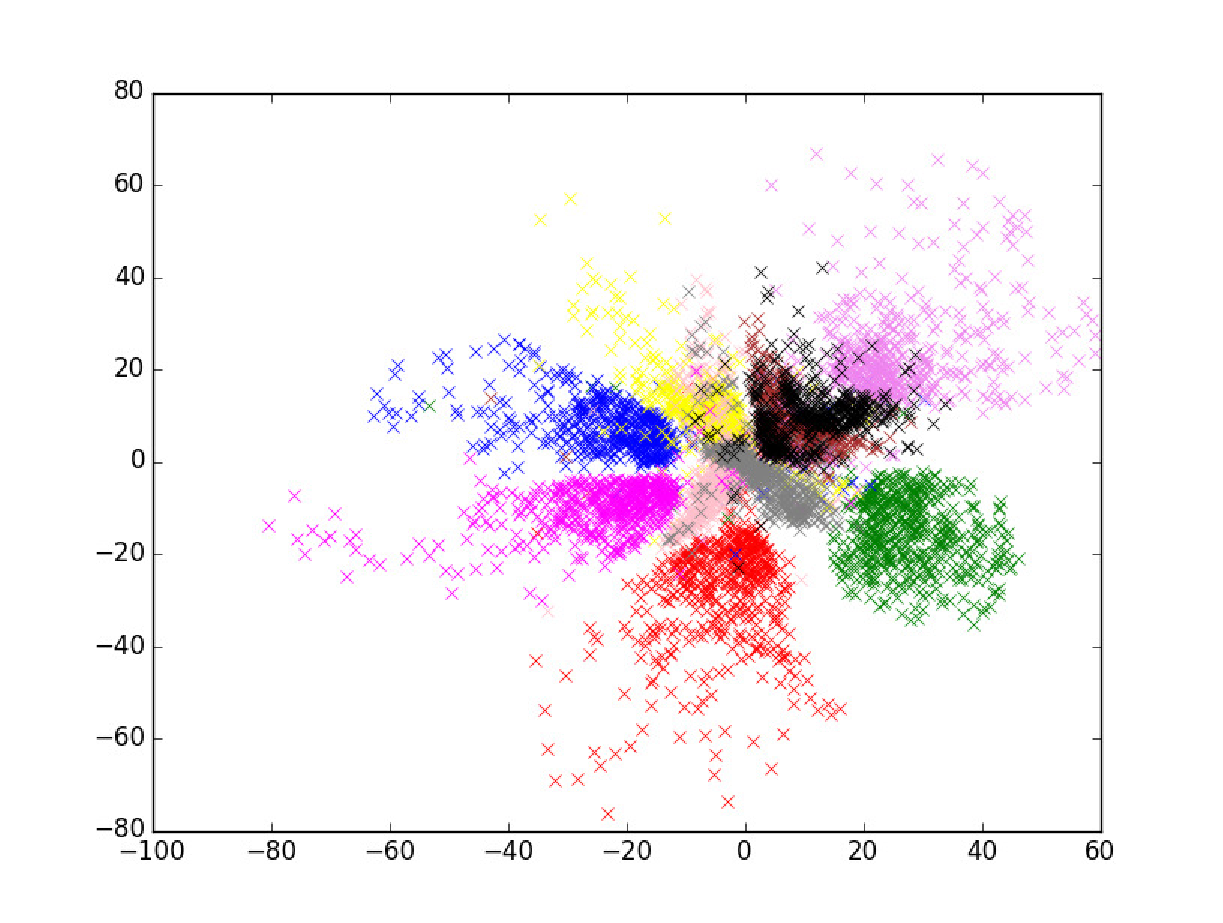
\includegraphics[width=16cm]{man-source/images/ch3/pic3-1.pdf}
% 	\caption{Визуализация рукописных цифр из базы MNIST}
% 	\label{fig:mnist_dataset_visualize}
% \end{figure}

% На рисунке видно, что в процессе обучения выделились кластеры в 2-ном пространстве главных компонент, соответствующие каждой цифре из оригинальной выборки. Таким образом, сеть не располагая информацией о каких-либо метках для исходных данных, смогла выделить области наибольшего подобия.

% \section{Семантическое кодирование}

% \subsection{Постановка задачи}
% В качестве обучающей выборки для решения задачи построения бинарных семантических кодов изображений нами была использована база CIFAR-10.  Данная выборка предоставляет богатый материал для выявления семантических особенностей \cite{n17}. Она включает в себя 50.000 изображений технических средств и живых существ, принадлежащий 10 различным классам (рис. \ref{fig:cifar_dataset}). Каждое изображение имеет размер 32Х32 пикселя.

% Помимо этого, CIFAR-10 включает тестирующую выборку, состоящую из 10.000 изображений.

% \begin{figure}[h]
% 	\begin{center}
% 		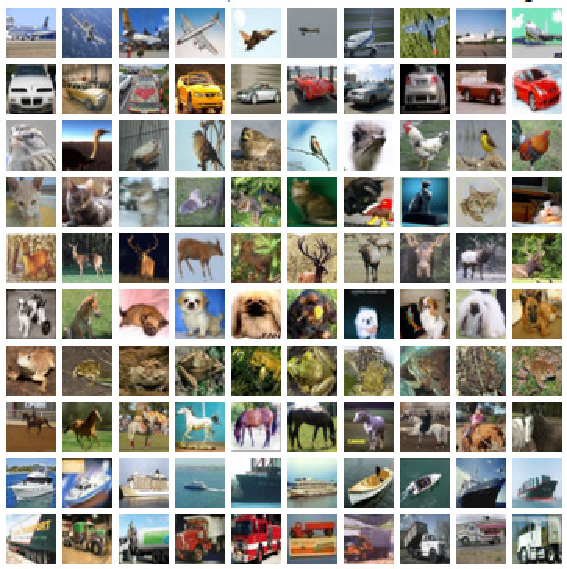
\includegraphics[width=12cm]{man-source/images/ch3/pic3-2.pdf}
% 		\caption{Фрагмент базы изображений CIFAR-10}				
% 		\label{fig:cifar_dataset}
% 	\end{center}
% \end{figure}

% Семантическое кодирование (хеширование) относится к более сложному и не менее важному типу задач, решение которого позволяет сформировать бинарный код ограниченной длины, емко и однозначно описывающий изображение в редуцированном признаковом пространстве. С помощью такого преобразования можно сформировать базу изображений, представленных лишь бинарным кодом. На основе такой базы можно построить систему релевантного поиска изображений.

% \subsection{Структура сети и основные параметры обучения}
% Для решения задачи нами использовалась 11-слойная ассоциативная нейронная сеть с архитектурой 3072-4096-2048-1024-512-256-512-1024-2048-4096-3072. На среднем слое такой сети формируется вектор вещественных значений из отрезка [0, 1], элементы которого затем округляются. Таким образом формируется бинарный код изображения. Легко видеть, что таким образом может быть закодировано $2^{256}$ изображений, что более чем достаточно для базы CIFAR-10. Нами использовались все изображения из обучающей выборки указанной базы.

% Обучение проводилось в два этапа. На первом этапе предобучались соответствующие RBM, формирующие кодирующие слои сети. Исходные данные перед обучением были стандартизованы: из каждого компонента вектора изображения вычиталось его среднее значение по всем изображениям выборки и затем полученное значение делилось на стандартное отклонение по всем компонентам всех изображений. Данное преобразование определило тип первой обучаемой машины Больцмана -- линейно-бинарная RBM \cite{n4}. Остальные машины обучались как бинарные RBM.

% Каждая RBM обучалась на протяжении 100 эпох мини-батчами по 100 элементов. Для линейно-бинарной RBM использовалось скорость обучения 0,001, для бинарной -- 0,01. Помимо этого для ускорения процесса обучения использовался моментный параметр, равный 0,9.

% После проведения предобучения выполнялось обучение развернутой автоассоциативной сети методом обратного распространения ошибки. Параметры обучения: скорость -- $1e^{-6}$, количество эпох обучения -- 150, моментный параметр -- 0.9.

% После выполнения обучения, результат оценивался вычислением расстояния Хэмминга между бинарными кодами для тестового изображения и изображениями из базы (формула \ref{chemming_dist}) После этого полученный ряд значений сортировался по возрастанию для выделения наиболее релевантных результатов.

% \begin{equation}
% 	\label{chemming_dist}
% 	H(v_1,v_2) = \sum_{i=1}^{n}|v_1^i-v_2^i|
% \end{equation}

% Вычисления, производимые в процессе обучения глубокой автоассоциативной нейронной сети производились на видеокарте GTX 750 Ti и заняли приблизительно 90 минут.

% Программный код на языке программирования Python для выполнения предобучения данной сети приведен в приложении 1.

% \subsection{Результаты обучения}
% Мы протестировали нашу модель двумя способами. Первый вариант предусматривал визуальное сравнение оригинального и восстановленного изображения. Некоторые из выполненных тестов представлены на рисунке \ref{fig:restore_images_results}.

% \begin{figure}[h]
% 	\begin{center}
% 		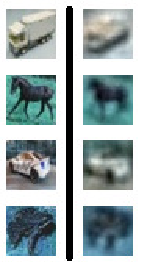
\includegraphics[width=40mm]{man-source/images/ch3/pic3-3.pdf}
% 		\caption{Оригинальные и восстановленные нейронной сетью изображения}				
% 		\label{fig:restore_images_results}
% 	\end{center}
% \end{figure}

% Второй вариант тестирования заключался в подаче на обученную автоассоциативную сеть изображения, получения его бинарного кода с промежуточного слоя сети и вычисления расстояния Хэмминга для всех остальных изображений. Отсортировав получившуюся последовательность по возрастанию, можно изучить наиболее релевантные результаты поиска (рис. \ref{fig:search_template}).

% \begin{figure}[h]
% 	\begin{center}
% 		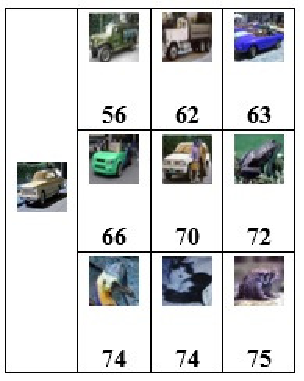
\includegraphics[width=8cm]{man-source/images/ch3/pic3-4.pdf}
% 		\caption{Поисковый шаблон и результаты поиска}				
% 		\label{fig:search_template}
% 	\end{center}
% \end{figure}

% Исходя из представленных данных, можно отметить, что с увеличением расстояния Хэмминга количество изображений того же класса, что и целевое изображение постепенно уменьшается.

\section{Редуцирование параметров НС}

Продемонстрируем эффективность предложенного подхода на примере редуцирования различных архитектур полносвязных нейронных сетей, применяемых для классификации изображений из выборок MNIST \cite{mnist}, CIFAR10 и CIFAR100 \cite{krizhevsky2009learning}.
Были проведены серии экспериментов, включающих различные используемые выборки, архитектуры и варианты предобучения. В рамках одной выборки и архитектуры НС текущая инициализация параметров сохранялась для возможности сравнения эффективности различных вариантов предобучающей процедуры.
Ниже для рассматриваемых выборок приведены основные параметры, включающие скорость обучения, размер мини-батча, моментный параметр и количество эпох для предобучения и <<тонкой настройки>> моделей (таблица \ref{table:reduce_training_params}).

\begin{table} [!h]
  \small
  \caption{Основные параметры обучения}\label{table:reduce_training_params}
\centering
\begin{tabular}{| p{3cm} | p{6cm} | p{2cm} |}
  \hline
    \textbf{Этап} & \textbf{Параметр} & \textbf{Значение}\\
    \hline
    Обучение & Скорость обучения & 0.05-0.1\\
    \cline{2-3}
    & Размер мини-батча & 100 \\
    \cline{2-3}
    & Моментный параметр & 0.9 \\
    \cline{2-3}
    & Количество эпох обучения & 50-100\\
    \hline
    Предобучение & Скорость обучения & 0.05-0.2\\
    \cline{2-3}
    & Размер мини-батча & 32-100 \\
    \cline{2-3}
    & Моментный параметр & [0.5, 0.9] \\
    \cline{2-3}
    & Количество эпох обучения & 10\\
    \hline
\end{tabular}
\end{table}

В результате вычислительного эксперимента были получены результаты для различных выборок, архитектур НС и значений параметра редуцирования t (таблицы \ref{table:mnist_1}-\ref{table:cifar_100}).

\begin{table} [!h]
  \small
  \caption{Результаты для сети 784-800-800-10 на выборке MNIST}\label{table:mnist_1}
\centering
\begin{tabular}{| p{2cm} | p{4cm} | p{4cm} | p{4cm} |}
  \hline
    \textbf{Тип} & \textbf{Эффективность, \%, C-RBM / REBA} & \textbf{Количество параметров, C-RBM / REBA} & \textbf{Редуцировано параметров, \%, C-RBM / REBA}\\
    \hline
    без редуц. & \textbf{98.63} / 98.33 & 1276810 / 1276810 & 0/0\\
    \hline
    t=0.2 & \textbf{98.61} / 98.27 & \textbf{233760} / 279635 & \textbf{81.69} / 78.1\\
    \hline
    t=0.5 & 98.03 / \textbf{98.05} & \textbf{32524} / 32817 & \textbf{97.45} / 97.43\\
    \hline
    t=0.8 & \textbf{97.1} / 96.48 & 17061 / \textbf{12217} & 98.66 / \textbf{99.04}\\
    \hline
\end{tabular}
\end{table}

\begin{table} [!h]
  \small
  \caption{Результаты для сети 784-1600-1600-800-800-10 на выборке MNIST}\label{table:mnist_2}
\centering
\begin{tabular}{| p{2cm} | p{4cm} | p{4cm} | p{4cm} |}
  \hline
    \textbf{Тип} & \textbf{Эффективность, \%, C-RBM / REBA} & \textbf{Количество параметров, C-RBM / REBA} & \textbf{Редуцировано параметров, \%, C-RBM / REBA}\\
    \hline
    wr & \textbf{98.76} / 98.37 & 5747210 / 5747210 & 0/0\\
    \hline
    t=0.2 & 98.51 / \textbf{98.55} & \textbf{710734} / 781103 & \textbf{87.63} / 86.41\\
    \hline
    t=0.5 & 98.01 / \textbf{98.03} & 54709 / \textbf{43867} & 99.05 / \textbf{99.24}\\
    \hline
    t=0.8 & \textbf{96.9} / 93.08 & 25385 / \textbf{14914} & 99.56 / \textbf{99.74}\\
    \hline
\end{tabular}
\end{table}

\begin{table} [!h]
  \small
  \caption{Результаты для сети 3072-1024-512-256-128-64-10 на выборке CIFAR10}\label{table:cifar_10_1}
\centering
\begin{tabular}{| p{2cm} | p{4cm} | p{4cm} | p{4cm} |}
  \hline
    \textbf{Тип} & \textbf{Эффективность, \%, C-RBM / REBA} & \textbf{Количество параметров, C-RBM / REBA} & \textbf{Редуцировано параметров, \%, C-RBM / REBA}\\
    \hline
    wr & \textbf{58.56} / 55.85 & 3844682 / 3844682 & 0/0\\
    \hline
    t=0.2 & \textbf{58.69} / 54.37 & 409211 / \textbf{227072} & 89.36 / \textbf{94.09}\\
    \hline
    t=0.5 & \textbf{42.08} / 41.2 & 29033 / \textbf{11320} & 99.24 / \textbf{99.71}\\
    \hline
    t=0.8 & \textbf{23.02} / 10.0 & 10058 / \textbf{4886} & 99.74 / \textbf{99.87}\\
    \hline
\end{tabular}
\end{table}

\begin{table} [!h]
  \small
  \caption{Результаты для сети 3072-512-256-128-64-10 на выборке CIFAR10 }\label{table:cifar_10_2}
\centering
\begin{tabular}{| p{2cm} | p{4cm} | p{4cm} | p{4cm} |}
  \hline
    \textbf{Тип} & \textbf{Эффективность, \%, C-RBM / REBA} & \textbf{Количество параметров, C-RBM / REBA} & \textbf{Редуцировано параметров, \%, C-RBM / REBA}\\
    \hline
    wr & \textbf{57.28} / 53.69 & 1746506 / 1746506 & 0/0\\
    \hline
    t=0.2 & \textbf{56.83} / 41.72 & 220037 / \textbf{126846} & 87.40 / \textbf{92.73}\\
    \hline
    t=0.5 & \textbf{45.29} / 44.93 & 20431 / \textbf{11383} & 98.83 / \textbf{99.35}\\
    \hline
    t=0.8 & 10.0 / 10.0 & 8599 / 3797 & 99.51 / 99.78\\
    \hline
\end{tabular}
\end{table}

\begin{table} [!h]
  \small
  \caption{Результаты для сети 3072-3072-1024-512-256-128-64-100 на выборке CIFAR100}\label{table:cifar_100}
\centering
\begin{tabular}{| p{2cm} | p{4cm} | p{4cm} | p{4cm} |}
  \hline
    \textbf{Тип} & \textbf{Эффективность, \%, C-RBM / REBA} & \textbf{Количество параметров, C-RBM / REBA} & \textbf{Редуцировано параметров, \%, C-RBM / REBA}\\
    \hline
    wr & 20.84 / \textbf{21.63} & 13290788 / 13290788 & 0/0\\
    \hline
    t=0.2 & 20.77 / \textbf{21.01} & 1304525 / \textbf{703319} & 90.18 / \textbf{94.71}\\
    \hline
    t=0.5 & \textbf{13.4} / 1.0 & 49847 / \textbf{24636} & 99.62 / \textbf{99.81}\\
    \hline
    t=0.8 & \textbf{2.67} / 1.0 & 21329 / \textbf{16977} & 99.84 / \textbf{99.87}\\
    \hline
\end{tabular}
\end{table}
% \begin{figure}[h]
% 	\begin{center}
% 		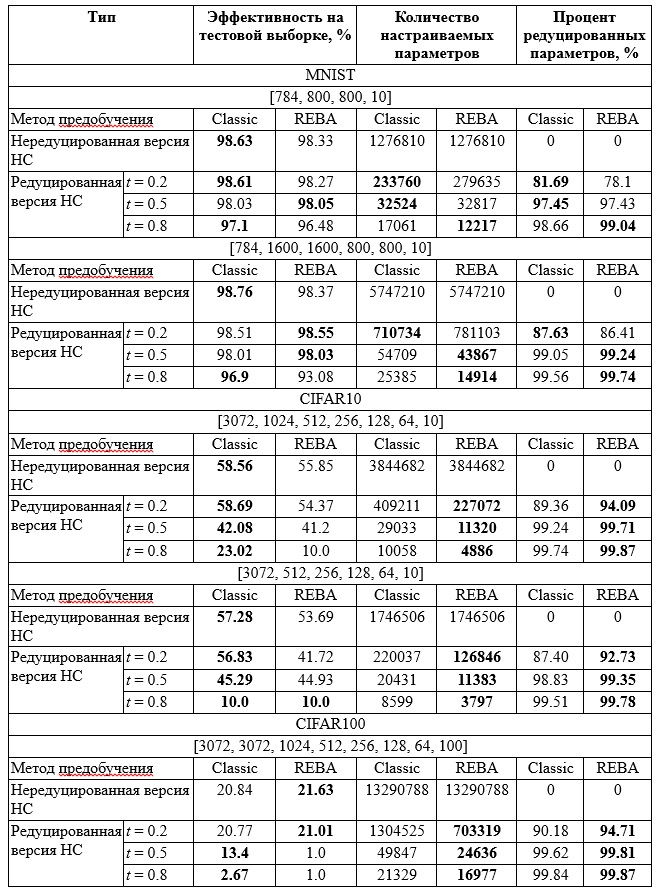
\includegraphics[width=18cm]{man-source/images/ch3/pic3-13.jpg}
% 		\caption{Результаты редуцирования}				
% 		\label{fig:reduce_results}
% 	\end{center}
% \end{figure}

Как видно из приведенных результатов, исследуемые архитектуры в целом сохраняют обобщающую способность, будучи редуцированными более чем на 80 процентов.

Также можно заметить, что чем больше настраиваемых параметров в модели, тем эффективней осуществляется редуцирование. Однако с увеличением параметра редуцирования эффективность исходной сети постепенно снижается, так как редуцированию начинают подвергаться параметры, наличие которых влияет на выходы нейронной сети.

Полученные результаты обосновывают возможность предобучения глубокой нейронной сети с использованием неконтролируемой процедуры без получения эффекта переобучения и снижения эффективности модели, так как в процессе предобучения фактически снижается влияние определенных параметров модели на итоговую выходную активность сети. Такие параметры имеют ``паразитический'' характер и фактически являются фактором переобучения модели. На этапе <<тонкой настройки>> модели они не модифицируются и могут быть удалены после этапа предобучения.
% Продемонстрируем эффективность предложенного подхода на примере редуцирования различных архитектур полносвязных нейронных сетей, применяемых для классификации изображений из выборок MNIST [12], CIFAR10 и CIFAR100 [13]. Данные выборки являются классическими для проверки эффективности моделей машинного обучения.
% Нами были проведены серии экспериментов, включающих различные используемые выборки, архитектуры и варианты предобучения. В рамках одной выборки и архитектуры НС текущая инициализация параметров сохранялась для возможности сравнения эффективности различных вариантов предобучающей процедуры.
% Ниже для рассматриваемых выборок приведены основные параметры, включающие скорость обучения, размер мини-батча, моментный параметр и количество эпох для предобучения и дообучения моделей (табл \ref{table:reduce_training_params}).

% \begin{table} [H]
%   \small
%   \caption{Основные параметры обучения}\label{table:reduce_training_params}
% \begin{tabularx}{\hsize}{| X | X | X |}
%   \hline
%     \multicolumn{2}{|c|}{\textbf{Функции активации}} &
%     \textbf{Сигмодные на все слоях, кроме последнего (линейная)}\\
%     \hline
%     \multirow{4}{*}{Обучение} & Скорость обучения & 0.05-0.1\\
%     \cline{2-3}
%     & Размер мини-батча & 100 \\
%     \cline{2-3}
%     & Моментный параметр & 0.9 \\
%     \cline{2-3}
%     & Количество эпох обучения & 50-100\\
%     \hline
%     \multirow{4}{*}{Предобучение} & Скорость обучения & 0.05-0.2\\
%     \cline{2-3}
%     & Размер мини-батча & 32-100 \\
%     \cline{2-3}
%     & Моментный параметр & [0.5, 0.9] \\
%     \cline{2-3}
%     & Количество эпох обучения & 10\\
%     \hline
% \end{tabularx}
% \end{table}

% В результате вычислительного эксперимента были получены результаты для различных архитектур НС и значений параметра редуцирования t (табл. \ref{fig:reduce_results}).

% \begin{figure}[h]
% 	\begin{center}
% 		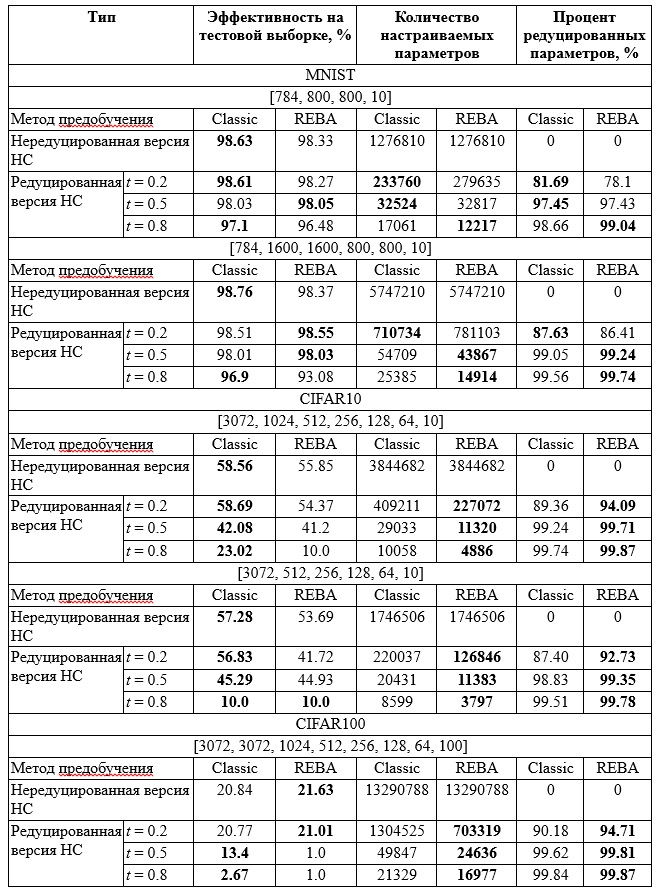
\includegraphics[width=18cm]{man-source/images/ch3/pic3-13.jpg}
% 		\caption{Результаты редуцирования}				
% 		\label{fig:reduce_results}
% 	\end{center}
% \end{figure}
% \begin{table} [H]
%   \small
%   \caption{Результаты редуцирования}\label{table:reduce_results}
% \begin{tabularx}{\hsize}{| X | X | X | X | X | X | X | X |}
%   \hline
%     \multicolumn{2}{|c|}{\textbf{Тип}} & &
%     \multicolumn{2}{|c|}{\textbf{Эффективность на тестовой выборке, \%}} & & \multicolumn{2}{|c|}{\textbf{Количество настраиваемых параметров}} & & \multicolumn{2}{|c|}{\textbf{Процент редуцированных параметров, \%}} &\\
%     \hline
%     \multicolumn{8}{|c|}{MNIST}\\
%     \hline
%     \multicolumn{8}{|c|}{[784, 800, 800, 10]}\\
%     \hline
%     \multicolumn{2}{|c|}{\textbf{Метод предобучения}} & Classic & REBA & Classic & REBA & Classic & REBA\\
%     % \cline{2-3}
%     % & Размер мини-батча & 100 \\
%     % \cline{2-3}
%     % & Моментный параметр & 0.9 \\
%     % \cline{2-3}
%     % & Количество эпох обучения & 50-100\\
%     % \hline
%     % \multirow{4}{}{Предобучение} & Скорость обучения & 0.05-0.2\\
%     % \cline{2-3}
%     % & Размер мини-батча & 32-100 \\
%     % \cline{2-3}
%     % & Моментный параметр & [0.5, 0.9] \\
%     % \cline{2-3}
%     % & Количество эпох обучения & 10\\
%     \hline
% \end{tabularx}
% \end{table}

Помимо редуцирования параметров, было выполнено так называемое архитектурное редуцирование (шаг 3 алгоритма), на котором производилось упрощение структуры слоев моделей за счет исключения нейронов с нулевыми векторами связей.

В следующих таблицах (\ref{table:architect_reduce_mnist_one}, \ref{table:architect_reduce_mnist_two}) приведены результаты архитектурного редуцирования для двух различных архитектур и обучающей выборки MNIST. Для предобучения использовался метод REBA.

\begin{table} [!h]
  \small
  \caption{Результаты для сети 784-800-800-10 на выборке MNIST}\label{table:architect_reduce_mnist_one}
    \centering
    \begin{tabular}{| p{2cm} | p{6cm} | p{6cm} |}
    \hline
        \textbf{Параметр} & \textbf{Исходная} & \textbf{Редуцированная}\\
    \hline
    t=0.2 & 784-800-800-10 & 784-800-556-10\\
    \hline
    t=0.5 & -//- & 784-710-422-10\\
    \hline
    t=0.9 & -//- & 784-91-114-10\\
    \hline
    \end{tabular}
    \end{table}
    
\begin{table} [!h]
  \small
    \caption{Результаты для сети 784-1600-1600-800-800-10 на выборке MNIST}\label{table:architect_reduce_mnist_two}
    \centering
    \begin{tabular}{| p{2cm} | p{6cm} | p{6cm} |}
    \hline
        \textbf{Параметр} & \textbf{Исходная} & \textbf{Редуцированная}\\
    \hline
    t=0.2 & 784-1600-1600-800-800-10 & 784-889-192-686-221-10\\
    \hline
    t=0.5 & -//- & 784-464-157-567-182-10\\
    \hline
    t=0.9 & -//- & 784-17-101-118-50-10\\
    \hline
    \end{tabular}
    \end{table}
    
Из приведенных таблиц можно заметить, что для моделей с большим количеством слоев и нейронов в каждом слое вероятность архитектурного редуцирования выше и оно начинает происходить уже для сравнительно небольших значений параметра редуцирования \textit{t}, в том время как для более <<поверхностных>> моделей оно существеннее проявляется только для больших значений параметра. Стоит отметить, что архитектуры, которые сохраняют почти все нейроны (например, \ref{table:architect_reduce_mnist_one}, архитектура при \textit{t}=0.2), все же при этом теряют для каждого нейрона основную часть связей (сохранение нейрона в данном случае будет иметь место, даже при сохранении одной связи нейрона с предыдущим слоем).

\section{Выводы}

\begin{easylistNum}
    & Проведен сравнительный анализ методов предобучения ГНС для задачи сжатия данных с использованием автоэнкодерной модели НС.
    & Проведен сравнительный анализ методов предобучения ГНС для задачи распознавания образов с использованием выборок MNIST, CIFAR-10 и CIFAR-100. Предложена модификация метода предобучения.
    %& Проведена серия экспериментов по визуализации данных выборки MNIST с применением предлагаемого метода предобучения.
    %& Проведены экспериментальные исследования по решению задачи семантического кодирования изображений из выборки CIFAR-10 с применением глубокой автоассоциативной нейронной сети и предлагаемого метода предобучения.
    & Проведены экспериментальные исследования редуцирования параметров глубокой нейронной сети с использованием различных методов предобучения и архитектур ГНС.
\end{easylistNum}
